\documentclass{article}
\usepackage{listings}
\usepackage{ctex}
\usepackage{graphicx}
\usepackage[a4paper, body={18cm,22cm}]{geometry}
\usepackage{amsmath,amssymb,amstext,wasysym,enumerate,graphicx,caption,subfigure}
\usepackage{float,abstract,booktabs,indentfirst,amsmath}
\usepackage{array}
\usepackage{booktabs} %调整表格线与上下内容的间隔
\usepackage{multirow}
\usepackage{url}
\usepackage{diagbox}
\renewcommand\arraystretch{1.4}
\usepackage{indentfirst}
\setlength{\parindent}{2em}
\usepackage{listings}
\usepackage{xcolor}
\lstset{
	numbers=left, 
	numberstyle= \tiny, 
	keywordstyle= \color{ blue!70},
	commentstyle= \color{red!50!green!50!blue!50}, 
	frame=shadowbox, % 阴影效果
	rulesepcolor= \color{ red!20!green!20!blue!20} ,
	escapeinside=``, % 英文分号中可写入中文
	xleftmargin=2em,xrightmargin=2em, aboveskip=1em,
	basicstyle=\footnotesize,
	framexleftmargin=2em
} 


\geometry{left=2.8cm,right=2.2cm,top=2.5cm,bottom=2.5cm}
%\geometry{left=3.18cm,right=3.18cm,top=2.54cm,bottom=2.54cm}

\graphicspath{{figures/}}

\title{\heiti 数字电路实验报告 }

\begin{document}
	\vspace*{1cm}
	
	\begin{figure}[h]
		\centering
		
\includegraphics[scale=1.0]{xh.jpg}
	\end{figure}

	\vspace*{0.5cm}
	
	\begin{center}
		\Huge{\textbf{数字电路实验报告}}
	\end{center}
	
	\vspace{5cm}
	
	\begin{table}[h]
		\centering
		\begin{Large}
			\begin{tabular}{p{3cm} p{7cm}<{\centering}}
				实验题目: &  简单时序逻辑电路     \\ \cline{2-2}
				学生姓名:      & 孔浩宇   \\ \cline{2-2}
				学生学号: & PB20000113 \\ \cline{2-2}
				完成日期:       & 2022/10/27 \\ \cline{2-2}
			\end{tabular}
		\end{Large}		
	\end{table}
	\newpage
    \section{实验题目}
        \subsection*{\qquad Verilog 简单时序逻辑电路}

    \section{实验目的}
        \subsection*{\qquad (1)掌握时序逻辑相关器件的原理及底层结构}
        \subsection*{\qquad (2)能够用基本逻辑门搭建各类时序逻辑器件}
        \subsection*{\qquad (3)能够使用 Verilog HDL 设计简单逻辑电路}
        
    \section{实验环境}
        \subsection*{\qquad (1) vlab.ustc.edu.cn}
        \subsection*{\qquad (2) Logisim}
        \subsection*{\qquad (3) verilogoj.ustc.edu.cn}
    
    \clearpage
    \section{实验练习}
    \subsection*{题目1}电路图及功能如图
    \begin{figure*}[htbp]
        \centering
        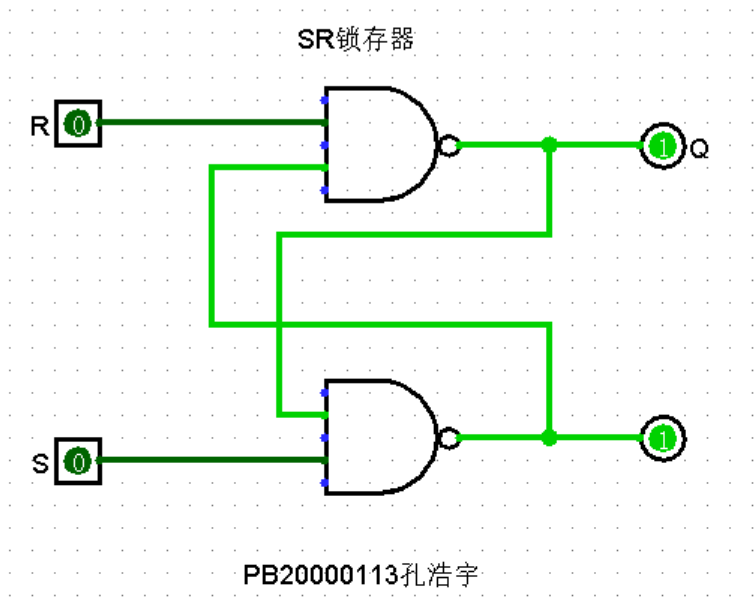
\includegraphics[scale=0.8]{t1.png}
        \caption*{SR锁存器}
    \end{figure*}
    \begin{figure*}[htbp]
        \centering
        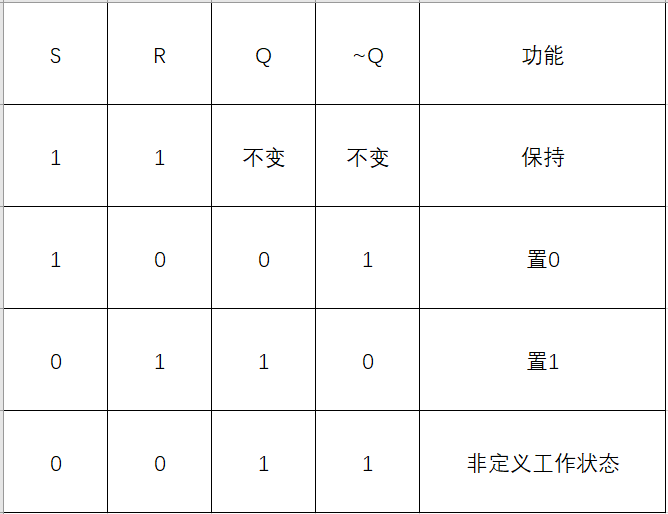
\includegraphics[scale=0.8]{t11.png}
        \caption*{电路状态}
    \end{figure*}

    \clearpage
    \subsection*{题目2} 先构造D锁存器如图
    \begin{figure*}[htbp]
        \centering
        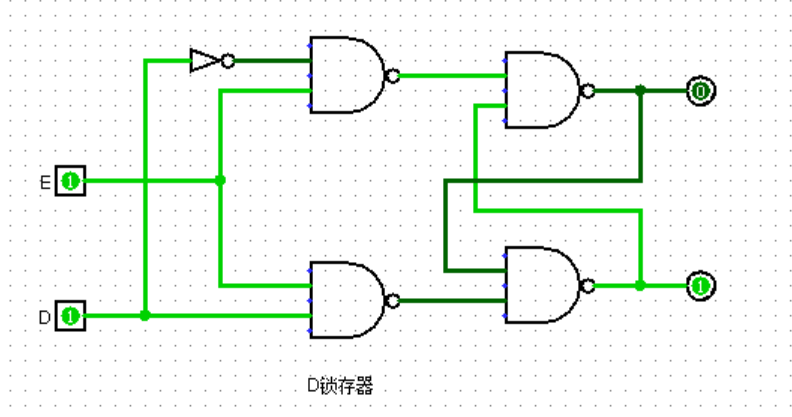
\includegraphics[scale=0.65]{t21.png}
        \caption*{D锁存器}
    \end{figure*}

    D触发器如图
    \begin{figure*}[htbp]
        \centering
        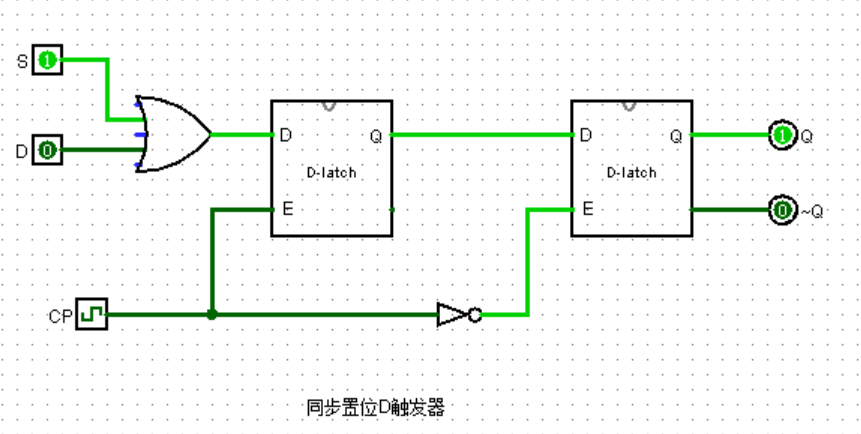
\includegraphics[scale=0.65]{t22.png}
        \caption*{同步置位D触发器}
    \end{figure*}

    Verilog代码如图
    \begin{figure*}[htbp]
        \centering
        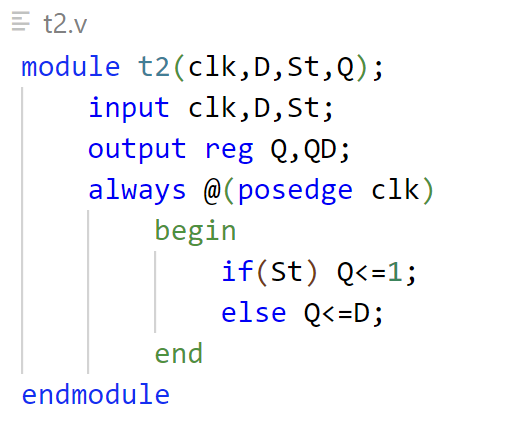
\includegraphics[scale=0.8]{t2v.png}
    \end{figure*}

    \clearpage
    \subsection*{题目3}
    异步复位D触发器如图
    \begin{figure*}[htbp]
        \centering
        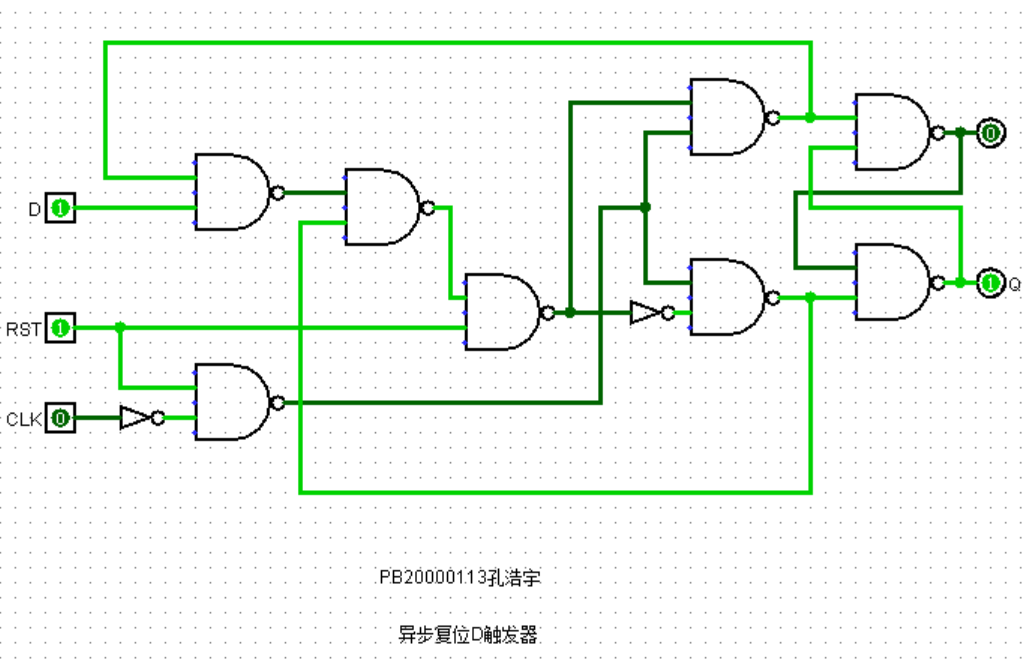
\includegraphics[scale=0.6]{t31.png}
        \caption*{异步复位D触发器}
    \end{figure*}

    递增计数器电路图如图
    \begin{figure*}[htbp]
        \centering
        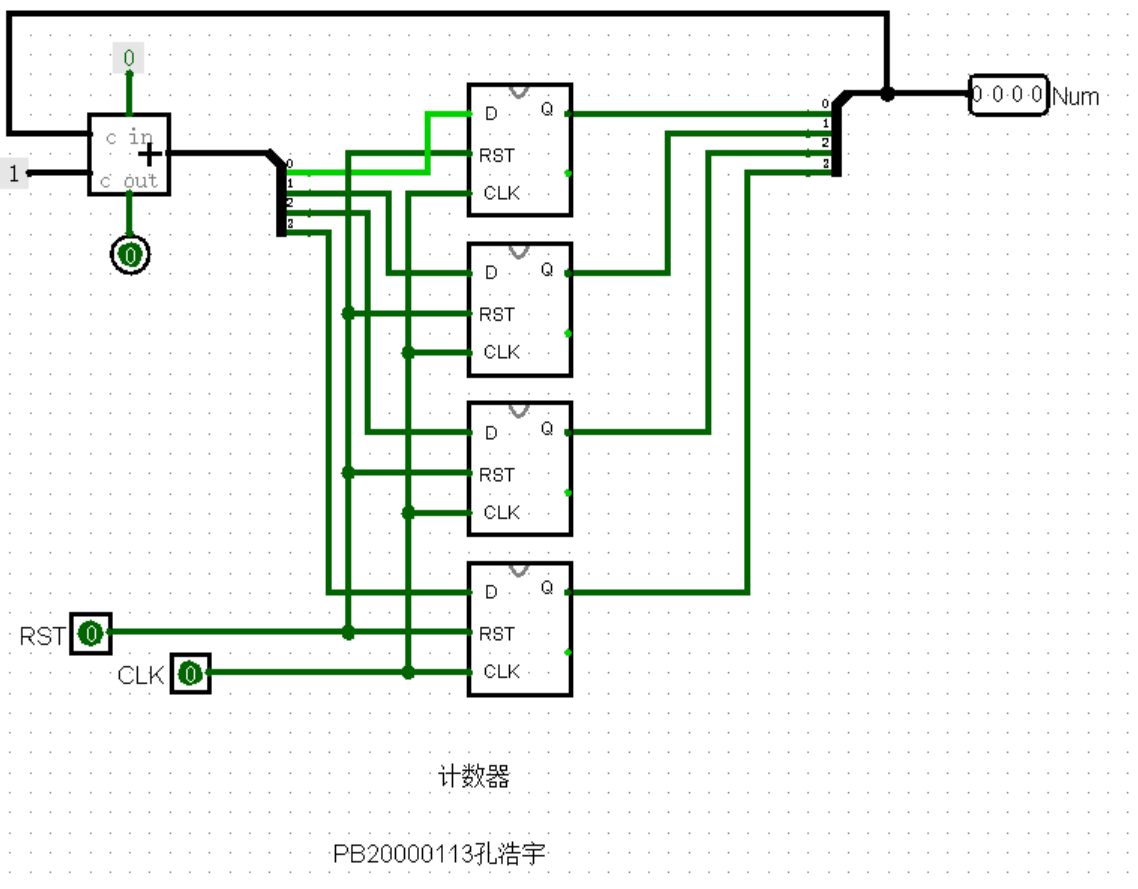
\includegraphics[scale=0.6]{t32.png}
        \caption*{递增计数器}
    \end{figure*}
    
    \clearpage
    Verilog代码如图
    \begin{figure*}[htbp]
        \centering
        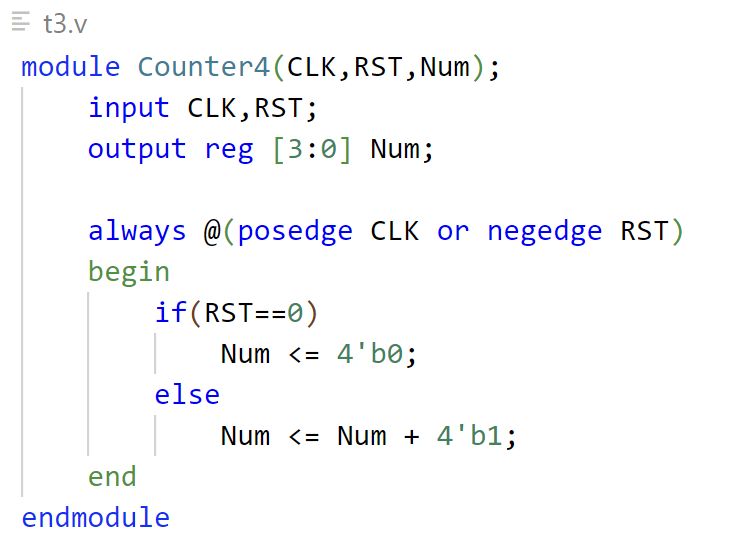
\includegraphics[scale=0.8]{t3v.png}
    \end{figure*}
    \vspace*{3cm}
    \subsection*{题目4}	
    首先搭建同步复位D触发器
    \begin{figure*}[htbp]
        \centering
        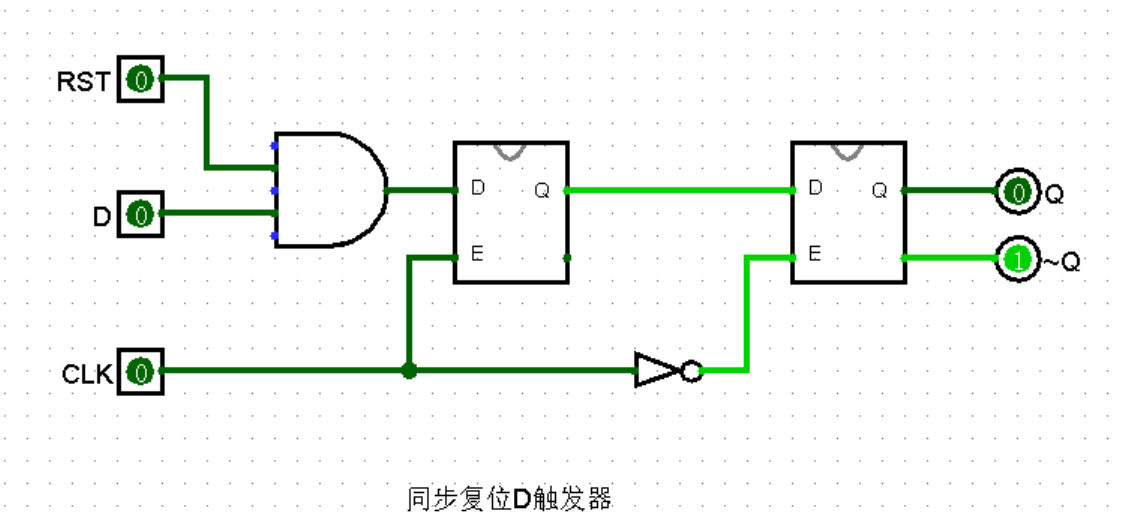
\includegraphics[scale=0.8]{t40.png}
        \caption*{同步复位D触发器}
    \end{figure*}
    \clearpage
    递减计数器如图
    \begin{figure*}[htbp]
        \centering
        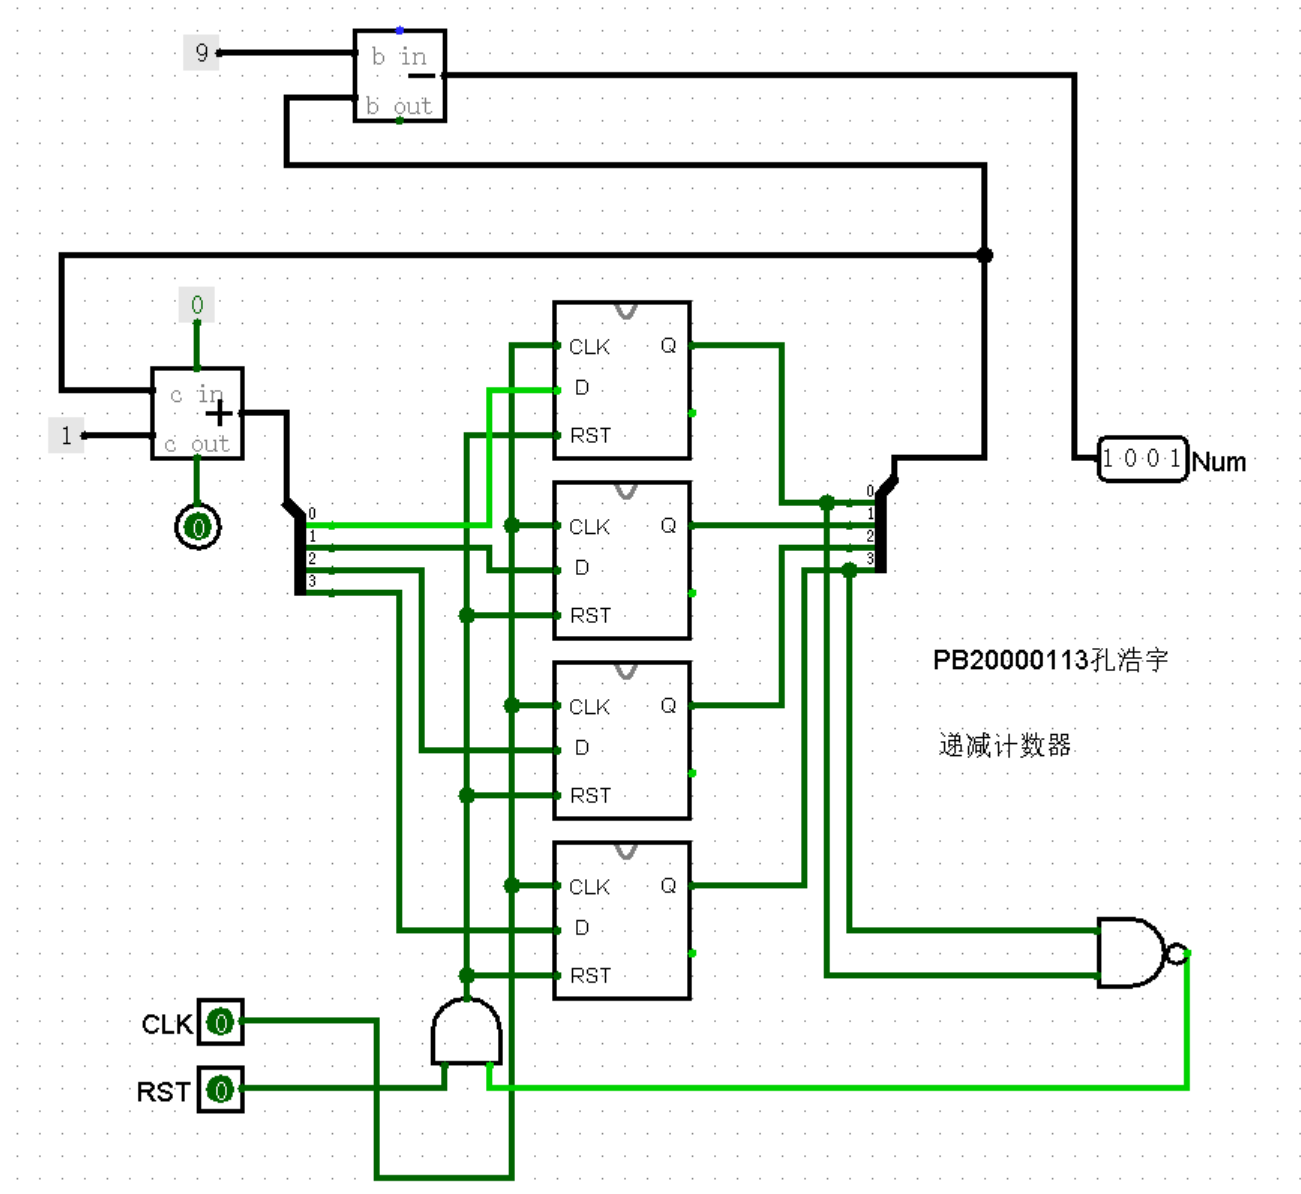
\includegraphics[scale=0.55]{t4.png}
    \end{figure*}

    Verilog代码如图
    \begin{figure*}[htbp]
        \centering
        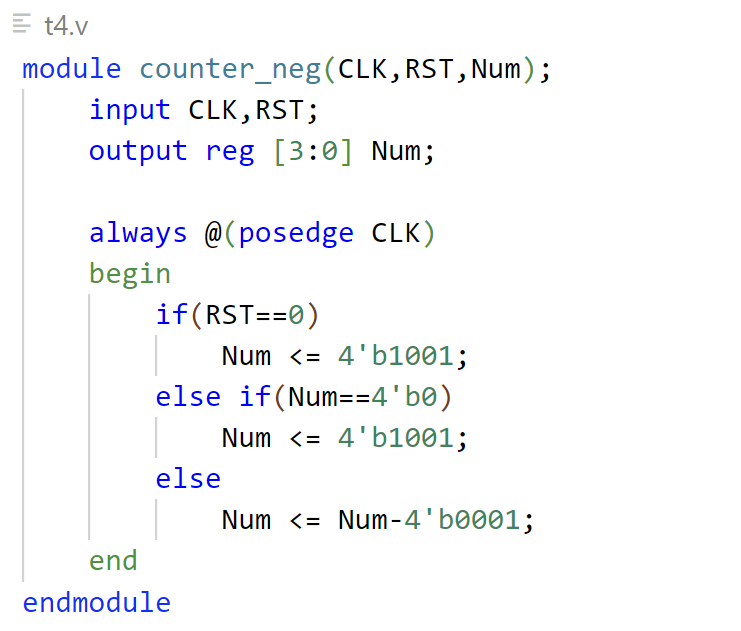
\includegraphics[scale=0.6]{t4v.png}
    \end{figure*}
    \clearpage
    \subsection*{题目5} 
    如图
    \begin{figure*}[htbp]
        \centering
        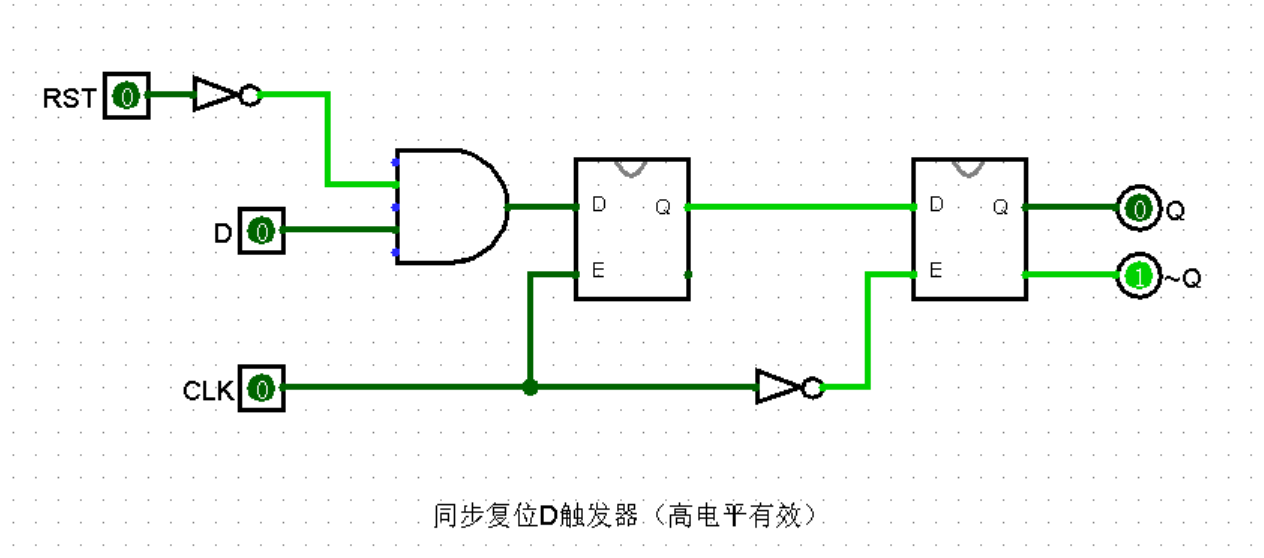
\includegraphics[scale=0.6]{t5.png}
    \end{figure*}

    Verilog代码如图
    \begin{figure*}[htbp]
        \centering
        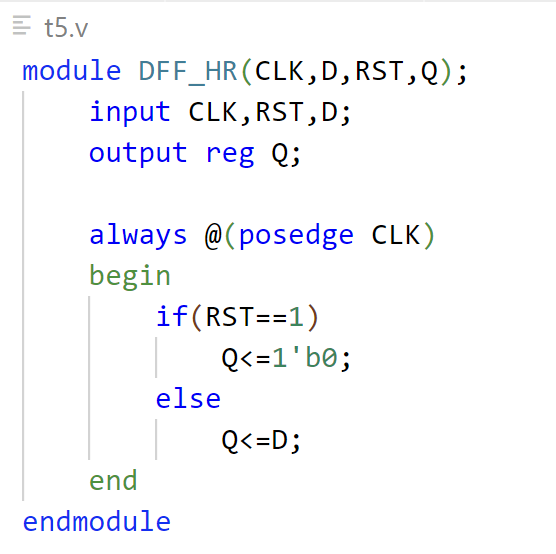
\includegraphics[scale=0.8]{t5v.png}
    \end{figure*}
    \clearpage
   \section{总结与思考}
    \begin{enumerate}
        \item [1.]学会了使用基本逻辑门搭建各类时序逻辑器件
        \item [2.]本次实验较难
        \item [3.]本次实验任务量较大
        \item [4.]经常出现奇怪的震荡错误,完全没有头绪
    \end{enumerate}
\end{document}